% ============================================================
% CNSH: A Human-Centered AI Governance and Knowledge Architecture
% IEEE Research Paper v4.0
% DNA   : #龍芯⚡️2026-03-17-CNSH-GOVERNANCE-IEEE-v4.0
% 作者   : UID9622 · 诸葛鑫·Lucky
% 编译命令: xelatex main.tex && xelatex main.tex && xelatex main.tex
% 依赖环境: TeX Live 2023+ / macOS Songti SC 字体
% 许可证  : CC BY-NC-SA 4.0
% GPG指纹 : A2D0092CEE2E5BA87035600924C3704A8CC26D5F
% 确认码  : #CONFIRM🌌9622-ONLY-ONCE🧬LK9X-772Z
% ============================================================

% ── 文档类 ─────────────────────────────────────────────────
\documentclass[conference]{IEEEtran}

% ── 字体与编码（XeLaTeX 专用）──────────────────────────────
\usepackage{fontspec}
\setmainfont{Songti SC}[
  BoldFont={Songti SC Bold},
  ItalicFont={Kaiti SC Regular}
]
\usepackage{amsmath,amssymb,amsthm}
\usepackage{graphicx}
\usepackage{booktabs}
\usepackage{hyperref}
\usepackage{cite}
\usepackage{algorithm}
\usepackage{algpseudocode}
\usepackage{tikz}
\usepackage{pgfplots}
\pgfplotsset{compat=1.18}
\usetikzlibrary{shapes.geometric,arrows.meta,positioning,
                fit,backgrounds,calc,matrix,decorations.pathreplacing}
\usepackage{xcolor}
\usepackage{url}
\usepackage{multirow}
\usepackage{array}
\usepackage{tcolorbox}
\tcbuselibrary{skins,breakable}
\usepackage{enumitem}

% ── 颜色 ────────────────────────────────────────────────────
\definecolor{cnsBlue}{RGB}{30,90,180}
\definecolor{cnsGreen}{RGB}{0,128,80}
\definecolor{cnsRed}{RGB}{180,30,30}
\definecolor{cnsGold}{RGB}{180,140,0}
\definecolor{cnsGray}{RGB}{80,80,100}
\definecolor{cnsOrange}{RGB}{204,85,0}

% ── 定理环境 ────────────────────────────────────────────────
\newtheorem{theorem}{Theorem}
\newtheorem{definition}{Definition}
\newtheorem{proposition}{Proposition}
\newtheorem{claim}{Claim}
\newtheorem{corollary}{Corollary}

% ════════════════════════════════════════════════════════════
\begin{document}
% ════════════════════════════════════════════════════════════

\title{\textbf{CNSH: A Human-Centered AI Governance\\
and Knowledge Architecture}\\
{\large With CNSH-64 Decision-State Model, CNSH-Lang Governance\\
Automation Language, and CNSH-OS Seven-Layer Blueprint}}

\author{
  \IEEEauthorblockN{
    \textbf{Zhuge Xin (Lucky)~UID9622}
  }
  \IEEEauthorblockA{
    \textit{LongHun System · Independent System Architect} \\
    uid9622@petalmail.com \\
    GPG: \texttt{A2D0092CEE2E5BA87035600924C3704A8CC26D5F} \\
    DNA: \texttt{\#龍芯⚡️2026-03-17-CNSH-GOVERNANCE-IEEE-v4.0}
  }
}

\maketitle

% ── 摘要 ────────────────────────────────────────────────────
\begin{abstract}
This paper introduces CNSH, a human-centered architecture designed for
AI-assisted knowledge systems and governance frameworks.
The architecture integrates ethical constraints, decision-state
reasoning models, and transparent audit structures to ensure that AI
systems remain accountable, interpretable, and aligned with human values.

CNSH proposes a three-layer governance structure consisting of a
Principle Layer (governance logic), a System Layer (data and automation),
and an Interaction Layer (human interface).
The framework combines symbolic decision-state modeling
(the CNSH-64 model with 8 base states composing 64 decision states),
structured knowledge management via knowledge cards and knowledge graphs,
and automated auditing mechanisms.

We further present \textbf{CNSH-Lang}, a governance automation language
with near-natural-language syntax and built-in audit mechanisms;
\textbf{CNSH-OS}, a seven-layer operating system blueprint for
human-centered AI collaboration; and the \textbf{CNSH System Constitution},
a seven-article constitutional framework establishing
the foundational principles of transparent, accountable AI governance.

The goal of CNSH is to create a \emph{transparent and resilient AI
collaboration environment}, enabling humans and intelligent systems
to operate within clear ethical and structural boundaries.
\end{abstract}

\begin{IEEEkeywords}
CNSH, AI governance, human-centered architecture, decision-state model,
knowledge graph, ethical constraint engine, audit system,
governance automation language, CNSH-Lang, CNSH-OS, system constitution
\end{IEEEkeywords}

% ════════════════════════════════════════════════════════════
\section{Introduction}
% ════════════════════════════════════════════════════════════

Modern AI systems are rapidly expanding in capability but often lack
transparent governance structures. Key challenges include:
\begin{itemize}[nosep]
  \item lack of traceable decision mechanisms,
  \item absence of ethical boundaries,
  \item fragmented knowledge systems,
  \item insufficient accountability in automated systems.
\end{itemize}

CNSH addresses these problems by introducing a unified architecture
that integrates ethical governance, symbolic reasoning structures,
transparent data systems, and human-centered interaction design.
The system does not attempt to replace human decision-making.
Instead, it focuses on \emph{augmenting human reasoning through
structured AI assistance}.

\subsection{Core Design Philosophy}

The CNSH framework follows five core design principles:

\begin{enumerate}[nosep]
  \item \textbf{Transparency}: All decisions and system actions
    must be traceable.
  \item \textbf{Responsibility}: Every automated action must have
    a verifiable origin.
  \item \textbf{Ethical Alignment}: System operations must remain
    within defined ethical boundaries.
  \item \textbf{Human Priority}: Technology serves people rather
    than replacing human judgment.
  \item \textbf{Knowledge Continuity}: Knowledge must remain
    understandable and maintainable over long time periods.
\end{enumerate}

\subsection{The Three-Layer Governance Architecture}

CNSH implements a hierarchical system architecture as shown in
Table~\ref{tab:threelayer}.

\begin{table}[t]
\centering
\caption{CNSH Three-Layer Governance Architecture}
\label{tab:threelayer}
\renewcommand{\arraystretch}{1.3}
\begin{tabular}{ll}
\toprule
\textbf{Layer} & \textbf{Function} \\
\midrule
Principle Layer & Governance logic and decision models \\
System Layer & Structured data and automation \\
Interaction Layer & Human interface and operational tools \\
\bottomrule
\end{tabular}
\end{table}

This separation improves maintainability, interpretability,
and system scalability.

% ════════════════════════════════════════════════════════════
\section{The CNSH-64 Decision-State Reasoning Model}
% ════════════════════════════════════════════════════════════

CNSH introduces a symbolic decision-state model to guide
AI-supported reasoning. The model represents operational states
of a system through 8 base states that combine to form
64 decision states.

\subsection{Base States}

\begin{table}[t]
\centering
\caption{CNSH-64 Base States}
\label{tab:basestates}
\renewcommand{\arraystretch}{1.2}
\begin{tabular}{cll}
\toprule
\textbf{State ID} & \textbf{Symbol} & \textbf{Meaning} \\
\midrule
S1 & Initiation & System creation or new action \\
S2 & Foundation & Structural foundation \\
S3 & Trigger & Event activation \\
S4 & Propagation & Communication or influence \\
S5 & Risk & Uncertainty detection \\
S6 & Awareness & Observation and analysis \\
S7 & Boundary & Limitation control \\
S8 & Cooperation & Coordinative interaction \\
\bottomrule
\end{tabular}
\end{table}

\subsection{State Composition}

States combine to form complex reasoning contexts.
For example:
\begin{itemize}[nosep]
  \item \textbf{Foundation + Trigger}: Stable system encountering change,
  \item \textbf{Risk + Boundary}: Potential threat under constraint,
  \item \textbf{Initiation + Cooperation}: New collaborative action.
\end{itemize}

These states function as \emph{reasoning primitives},
allowing complex situations to be interpreted through
structured symbolic states.

\subsection{Decision Flow}

The CNSH-64 decision flow follows a six-stage pipeline:

\begin{enumerate}[nosep]
  \item \textbf{Input Event}: Receive and parse external event,
  \item \textbf{State Identification}: Map event to base state(s),
  \item \textbf{State Combination}: Compose 64-state model,
  \item \textbf{Governance Evaluation}: Apply governance rules,
  \item \textbf{Ethical Constraint Check}: Validate ethical compliance,
  \item \textbf{Action Classification}: Output decision level.
\end{enumerate}

\subsection{Decision Classification}

\begin{table}[t]
\centering
\caption{Decision Classification Levels}
\label{tab:classification}
\renewcommand{\arraystretch}{1.2}
\begin{tabular}{cl}
\toprule
\textbf{Level} & \textbf{Result} \\
\midrule
\textcolor{cnsGreen}{🟢 Green} & Safe to execute \\
\textcolor{cnsGold}{🟡 Yellow} & Conditional execution \\
\textcolor{cnsRed}{🔴 Red} & Blocked or restricted \\
\bottomrule
\end{tabular}
\end{table}

\subsection{Automation Trigger Tags}

\begin{table}[t]
\centering
\caption{Automation Trigger Tags}
\label{tab:tags}
\renewcommand{\arraystretch}{1.2}
\begin{tabular}{cl}
\toprule
\textbf{Tag} & \textbf{Function} \\
\midrule
\texttt{\#decision} & Decision record \\
\texttt{\#risk} & Risk identification \\
\texttt{\#alert} & System warning \\
\texttt{\#governance} & Governance action \\
\texttt{\#audit} & Audit record \\
\bottomrule
\end{tabular}
\end{table}

% ════════════════════════════════════════════════════════════
\section{Ethical Constraint Engine}
% ════════════════════════════════════════════════════════════

A built-in ethical constraint engine evaluates actions before
execution. Evaluation dimensions include:
\begin{itemize}[nosep]
  \item social impact,
  \item operational risk,
  \item ethical compliance.
\end{itemize}

Results are categorized using the three-level classification
system described in Section~\ref{tab:classification}.
This model provides a lightweight but effective governance
structure for automated systems.

\begin{proposition}[Ethical Constraint Completeness]
For any system action $a$, the ethical constraint engine
$\mathcal{E}$ produces a classification
$\mathcal{E}(a) \in \{\text{GREEN}, \text{YELLOW}, \text{RED}\}$
such that:
\begin{equation}
  \mathcal{E}(a) = \text{RED} \implies a \text{ is blocked}
\end{equation}
and:
\begin{equation}
  \mathcal{E}(a) = \text{YELLOW} \implies a \text{ requires
    additional human review}.
\end{equation}
\end{proposition}

% ════════════════════════════════════════════════════════════
\section{Knowledge Architecture}
% ════════════════════════════════════════════════════════════

CNSH uses a structured knowledge-card system as its
fundamental knowledge unit.

\subsection{Knowledge Card Structure}

Each knowledge unit includes:
\begin{itemize}[nosep]
  \item title,
  \item summary,
  \item source,
  \item content,
  \item tags,
  \item relationships.
\end{itemize}

Knowledge cards form a \textbf{knowledge graph}, enabling
large-scale information organization and semantic retrieval.

\subsection{Knowledge Graph}

The knowledge graph $\mathcal{G} = (V, E, W)$ consists of:
\begin{itemize}[nosep]
  \item \textbf{Nodes} $V$: knowledge cards, decisions, events, resources,
  \item \textbf{Edges} $E$: references, influences, dependencies,
  \item \textbf{Weights} $W$: semantic proximity scores.
\end{itemize}

% ════════════════════════════════════════════════════════════
\section{Audit and Traceability}
% ════════════════════════════════════════════════════════════

All system actions generate audit records.
Each record contains:
\begin{itemize}[nosep]
  \item event ID,
  \item action type,
  \item operator,
  \item timestamp,
  \item result.
\end{itemize}

This ensures transparency, accountability, and forensic
analysis capability.

\begin{proposition}[Audit Completeness]
For every system operation $op$, there exists a unique
audit record $r_{op}$ such that:
\begin{equation}
  \forall op \in \mathcal{O}: \exists! r_{op} \in \mathcal{R}
  \quad \text{where} \quad
  r_{op} = (\text{id}, \text{type}, \text{operator},
    \text{timestamp}, \text{result})
\end{equation}
where $\mathcal{O}$ is the set of all operations and
$\mathcal{R}$ is the audit record set.
\end{proposition}

% ════════════════════════════════════════════════════════════
\section{Automation and System Health}
% ════════════════════════════════════════════════════════════

Automated monitoring maintains system integrity.
Monitoring includes:
\begin{itemize}[nosep]
  \item schema consistency,
  \item data completeness,
  \item duplicate detection,
  \item orphan node detection,
  \item broken relation detection.
\end{itemize}

When issues are detected, automated repair tasks are generated
with priority levels and notification mechanisms.

\subsection{System Health Cycle}

The health monitoring loop operates continuously:

\begin{enumerate}[nosep]
  \item \textbf{Scan}: Inspect all system components,
  \item \textbf{Detect}: Identify anomalies and issues,
  \item \textbf{Repair}: Generate and execute repair tasks,
  \item \textbf{Verify}: Confirm issue resolution.
\end{enumerate}

\subsection{Three Automation Cycles}

CNSH implements three continuous automation cycles:

\subsubsection{Knowledge Cycle}
\begin{quote}
input content $\to$ clean $\to$ summarize $\to$ tag
$\to$ store $\to$ connect graph
\end{quote}

\subsubsection{Governance Cycle}
\begin{quote}
event $\to$ evaluate state $\to$ ethical check
$\to$ decision classification $\to$ record audit
\end{quote}

\subsubsection{System Health Cycle}
\begin{quote}
scan system $\to$ detect anomalies $\to$ generate repair tasks
$\to$ verify fixes
\end{quote}

% ════════════════════════════════════════════════════════════
\section{CNSH-Lang: Governance Automation Language}
% ════════════════════════════════════════════════════════════

CNSH-Lang is a governance automation language designed for
human readability and built-in audit mechanisms.
Its core characteristics include:
\begin{itemize}[nosep]
  \item near-natural-language syntax,
  \item built-in governance and audit mechanisms,
  \item explicit constraint declaration,
  \item automated task scheduling.
\end{itemize}

\subsection{Action Declaration}

\begin{verbatim}
ACTION create_knowledge
  INPUT article
  OUTPUT knowledge_card
  TAG #learning
\end{verbatim}

\subsection{Decision Rule}

\begin{verbatim}
RULE evaluate_risk
  IF risk_score > 70
    THEN classification = RED
  ELSE classification = GREEN
\end{verbatim}

\subsection{Governance Constraint}

\begin{verbatim}
CONSTRAINT ethical_check
  IF action_impact = high
    REQUIRE human_review
\end{verbatim}

\subsection{Knowledge Conversion Pipeline}

\begin{verbatim}
PROCESS learning_pipeline
  INPUT raw_content
  STEP clean_text
  STEP summarize
  STEP generate_card
  STEP tag
  STEP store_database
\end{verbatim}

\subsection{Automated Task}

\begin{verbatim}
TASK system_health_scan
  RUN every 24h
  CHECK
    database_integrity
    orphan_nodes
    missing_properties
    duplicate_cards
\end{verbatim}

\subsection{Audit Record Format}

\begin{verbatim}
AUDIT_LOG
  event_id
  operator
  timestamp
  action_type
  result
\end{verbatim}

% ════════════════════════════════════════════════════════════
\section{CNSH-OS: Seven-Layer Operating System Blueprint}
% ════════════════════════════════════════════════════════════

CNSH-OS is a human-centered AI operating system architecture
designed for the AI collaboration era.
Its core goal is not to replace traditional systems, but to provide
a unified runtime environment for AI governance, knowledge management,
and automated collaboration.

\subsection{Seven-Layer Architecture}

\begin{figure}[t]
\centering
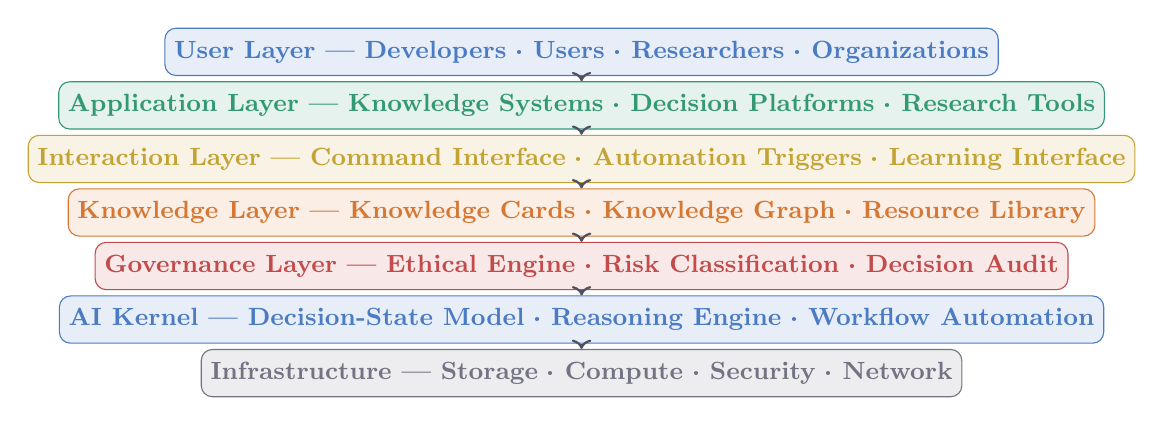
\begin{tikzpicture}[
  box/.style={rectangle, rounded corners=4pt, draw=#1!80,
              fill=#1!10, minimum width=7.2cm,
              minimum height=0.6cm, font=\small\bfseries,
              text=#1!80},
  arr/.style={->, thick, cnsGray},
  node distance=0.68cm
]
  \node[box=cnsBlue]   (L1) {User Layer --- Developers · Users ·
    Researchers · Organizations};
  \node[box=cnsGreen, below of=L1]  (L2)
    {Application Layer --- Knowledge Systems · Decision Platforms ·
     Research Tools};
  \node[box=cnsGold, below of=L2]   (L3)
    {Interaction Layer --- Command Interface · Automation Triggers ·
     Learning Interface};
  \node[box=cnsOrange, below of=L3] (L4)
    {Knowledge Layer --- Knowledge Cards · Knowledge Graph ·
     Resource Library};
  \node[box=cnsRed, below of=L4]    (L5)
    {Governance Layer --- Ethical Engine · Risk Classification ·
     Decision Audit};
  \node[box=cnsBlue, below of=L5]   (L6)
    {AI Kernel --- Decision-State Model · Reasoning Engine ·
     Workflow Automation};
  \node[box=cnsGray, below of=L6]   (L7)
    {Infrastructure --- Storage · Compute · Security · Network};
  \foreach \a/\b in {L1/L2,L2/L3,L3/L4,L4/L5,L5/L6,L6/L7}
    \draw[arr] (\a.south) -- (\b.north);
\end{tikzpicture}
\caption{CNSH-OS seven-layer system architecture.
  Each layer is independently extensible with clearly defined
  responsibilities.}
\label{fig:osarch}
\end{figure}

\subsection{AI Kernel}

The AI Kernel is the core engine of CNSH-OS, containing
four critical sub-modules:
\begin{itemize}[nosep]
  \item \textbf{State Model}: The CNSH-64 decision-state model,
  \item \textbf{Reasoning Engine}: Symbolic reasoning over
    combined states,
  \item \textbf{Workflow Automation}: Event-driven workflow
    scheduling,
  \item \textbf{Learning Processor}: Knowledge extraction
    and structuring.
\end{itemize}

\subsection{Governance Kernel}

The Governance Kernel distinguishes CNSH-OS from traditional
AI systems. Its core responsibilities include:
AI behavior constraint, decision transparency, and risk control.

The governance pipeline:
\begin{quote}
action request $\to$ risk evaluation $\to$ ethical validation
$\to$ decision classification $\to$ execution or block
$\to$ audit log
\end{quote}

\subsection{Knowledge Kernel}

The knowledge layer is the source of long-term system value.
Knowledge units are organized as Knowledge Cards with fields:
summary, content, source, tags, and relations.
Cards form a knowledge graph for semantic navigation.

\subsection{Identity Kernel}

The identity system ensures:
\begin{itemize}[nosep]
  \item unique user identification,
  \item clear permission levels,
  \item auditable contribution records.
\end{itemize}

Identity fields include: \texttt{identity\_id}, \texttt{dna\_hash},
\texttt{public\_key}, \texttt{access\_level},
\texttt{contribution\_score}.

\subsection{Automation Engine}

\begin{quote}
event trigger $\to$ state evaluation $\to$ workflow selection
$\to$ execution $\to$ audit recording
\end{quote}

Automation modules: workflow scheduler, trigger system,
repair engine, monitoring engine.

\subsection{Security Architecture}

\begin{itemize}[nosep]
  \item identity verification,
  \item access control,
  \item audit monitoring,
  \item policy enforcement.
\end{itemize}

\subsection{Application Scenarios}

CNSH-OS supports diverse domains:
\begin{itemize}[nosep]
  \item AI governance systems,
  \item research knowledge management,
  \item enterprise decision platforms,
  \item education systems,
  \item open-source communities.
\end{itemize}

\subsection{Future Extensions}

\begin{itemize}[nosep]
  \item distributed knowledge networks,
  \item local AI model integration,
  \item open-source ecosystem,
  \item cross-organization collaboration systems.
\end{itemize}

% ════════════════════════════════════════════════════════════
\section{CNSH System Constitution}
% ════════════════════════════════════════════════════════════

The CNSH Constitution defines the foundational principles,
governance mechanisms, and technical boundaries of the system.
Its goal is to ensure that technological development always
serves human society and remains transparent, fair, and accountable.

\subsection{Article 1 --- Human Priority}

The primary goal of technology is to \emph{enhance human capability}.
No automated system may diminish human decision-making authority
or agency. AI provides assistance; humans retain final judgment.
Important decisions must allow human intervention.

\subsection{Article 2 --- Transparency}

System behavior must remain interpretable.
Every system action must be traceable to:
behavior origin, execution logic, result record.
Transparency is achieved through the Audit System.

\subsection{Article 3 --- Accountability}

All system actions must produce verifiable records including:
operating subject, action type, execution time, execution result.
These records constitute the system's accountability mechanism.

\subsection{Article 4 --- Ethical Boundary}

Technical behavior must be constrained by ethics.
The Ethical Engine evaluates actions on:
risk level, social impact, ethical compliance.
High-risk actions require human review.

\subsection{Article 5 --- Knowledge Continuity}

The system must protect and perpetuate knowledge.
Knowledge structures must have:
long-term readability, traceable sources, clear structure.
Knowledge is stored as Knowledge Cards forming a knowledge network.

\subsection{Article 6 --- Responsible Automation}

Automation must be governed:
\begin{quote}
event trigger $\to$ governance evaluation $\to$ ethical validation
$\to$ execution $\to$ audit record
\end{quote}

\subsection{Article 7 --- System Integrity}

The system must possess self-detection capability.
Regular checks include:
data integrity, system structure, data relationships.
Issues automatically generate repair tasks.

% ════════════════════════════════════════════════════════════
\section{AI Governance Standard Proposal}
% ════════════════════════════════════════════════════════════

This section proposes a basic framework for AI system governance,
structured similarly to ISO/IEEE standards.

\subsection{Governance Framework}

AI systems should include four governance components:

\begin{table}[t]
\centering
\caption{Required Governance Components}
\label{tab:govcomponents}
\renewcommand{\arraystretch}{1.2}
\begin{tabular}{ll}
\toprule
\textbf{Component} & \textbf{Function} \\
\midrule
Audit System & Behavior tracking \\
Human Oversight & Human supervision \\
Ethical Engine & Constraint validation \\
Decision Model & State reasoning \\
\bottomrule
\end{tabular}
\end{table}

\subsection{Decision Governance Model}

\begin{quote}
input $\to$ context analysis $\to$ risk evaluation
$\to$ ethical validation $\to$ decision classification
$\to$ execution
\end{quote}

\subsection{Risk Classification}

\begin{table}[t]
\centering
\caption{AI Risk Classification Standard}
\label{tab:risklevels}
\renewcommand{\arraystretch}{1.2}
\begin{tabular}{cl}
\toprule
\textbf{Level} & \textbf{Handling} \\
\midrule
\textcolor{cnsGreen}{🟢 Low} & Normal execution \\
\textcolor{cnsGold}{🟡 Medium} & Monitored execution \\
\textcolor{cnsRed}{🔴 High} & Human review required \\
\bottomrule
\end{tabular}
\end{table}

\subsection{AI Accountability}

AI systems must possess:
\begin{itemize}[nosep]
  \item behavior records,
  \item explanation capability,
  \item traceable decisions.
\end{itemize}

\subsection{Human Oversight}

Any automated system must allow:
\begin{itemize}[nosep]
  \item pause execution,
  \item modify decisions,
  \item force termination.
\end{itemize}

\subsection{Governance Audit}

Periodic governance audit checks:
\begin{itemize}[nosep]
  \item AI behavior records,
  \item decision quality,
  \item risk management.
\end{itemize}

% ════════════════════════════════════════════════════════════
\section{CNSH Core Principle \& Technology Declaration}
% ════════════════════════════════════════════════════════════

\subsection{Core Declaration}

\begin{quote}
\textbf{Technology should enhance human capability while remaining
transparent, accountable, and ethically bounded.}
\end{quote}

\subsection{Principle-to-System Mapping}

\begin{table}[t]
\centering
\caption{Principle-to-System Module Mapping}
\label{tab:principlemap}
\renewcommand{\arraystretch}{1.3}
\begin{tabular}{ll}
\toprule
\textbf{Principle} & \textbf{System Module} \\
\midrule
Transparency & Audit System \\
Accountability & DNA Traceability \\
Ethical Boundary & Ethical Engine \\
Human Priority & Human Override Interface \\
\bottomrule
\end{tabular}
\end{table}

\subsection{System Enforcement Pipeline}

\begin{quote}
User Request $\to$ AI Assistance $\to$ Ethical Validation
$\to$ Execution $\to$ Audit Record
\end{quote}

\subsection{Engineering Rules}

\begin{enumerate}[nosep]
  \item AI does not directly replace human decision-making.
  \item All system behavior must be recorded.
  \item Any high-risk action must pass through the governance module.
  \item Automation must allow human intervention.
\end{enumerate}

\subsection{Governance Control}

\begin{quote}
action $\to$ risk evaluation $\to$ ethical validation
$\to$ approval or block
\end{quote}

\subsection{Transparency Mechanism}

All behavior is written to the Audit Log with fields:
action, operator, timestamp, result.

\subsection{Human Override}

Three override levels:
\begin{itemize}[nosep]
  \item \textbf{pause}: Temporarily halt execution,
  \item \textbf{modify}: Alter decision parameters,
  \item \textbf{cancel}: Force termination.
\end{itemize}

\subsection{Extended Governance Principles}

\begin{itemize}[nosep]
  \item \textbf{Knowledge Preservation}: Knowledge must be
    accumulable and traceable.
  \item \textbf{Responsible Automation}: Automation must be governed.
  \item \textbf{Human Sovereignty}: Final decision authority
    belongs to humans.
\end{itemize}

\subsection{Technology Declaration}

\begin{quote}
Technology must serve humanity.
Artificial intelligence should augment human capability rather
than replace human judgment.
Systems must remain transparent, accountable, and governed
by ethical boundaries.
Innovation without responsibility leads to instability.
Responsible technology creates sustainable progress.
\end{quote}

\subsection{Core Beliefs}

\begin{itemize}[nosep]
  \item Human values first,
  \item Technology must be governable,
  \item Knowledge must be openly accumulated,
  \item Innovation must bear responsibility.
\end{itemize}

\subsection{Vision}

CNSH's goal is to establish a new technological environment
for human-intelligent-system collaboration, in which:
humans maintain agency, AI provides capability extension,
systems remain transparent, and knowledge continuously accumulates.

\subsection{Core Formula}

\begin{equation}
\text{AI Capability}
+ \text{Human Judgment}
+ \text{Ethical Governance}
= \text{Responsible Intelligence}
\label{eq:coreformula}
\end{equation}

\subsection{System Motto}

\begin{quote}
\textbf{Human first. Technology accountable. Intelligence governed.}
\end{quote}

% ════════════════════════════════════════════════════════════
\section{Applications}
% ════════════════════════════════════════════════════════════

CNSH can support various domains:

\begin{itemize}[nosep]
  \item \textbf{Research knowledge systems}: Structured knowledge
    management with semantic retrieval,
  \item \textbf{AI governance platforms}: Ethical constraint
    enforcement and decision auditing,
  \item \textbf{Enterprise decision systems}: Transparent
    decision-state tracking,
  \item \textbf{Education platforms}: Knowledge card-based
    learning with graph navigation,
  \item \textbf{Open knowledge communities}: Collaborative
    knowledge accumulation with provenance tracking.
\end{itemize}

% ════════════════════════════════════════════════════════════
\section{Conclusion}
% ════════════════════════════════════════════════════════════

CNSH proposes a human-centered architecture for AI governance
and knowledge management.

By combining symbolic reasoning models (CNSH-64), ethical
constraints, transparent audit systems, and a governance
automation language (CNSH-Lang), CNSH aims to create AI systems
that remain accountable, interpretable, and aligned with
human values.

The seven-layer CNSH-OS blueprint provides a practical
engineering framework, while the CNSH System Constitution
establishes foundational principles that ensure technology
always serves humanity.

The core formula (Eq.~\ref{eq:coreformula}) captures the
essential insight: responsible intelligence emerges from the
combination of AI capability, human judgment, and ethical
governance---not from any single component alone.

Future work will explore distributed deployment, integration
with local AI models, and open-source collaboration.

\begin{quote}
\itshape
Human first. Technology accountable. Intelligence governed.
\end{quote}

% ════════════════════════════════════════════════════════════
\section*{Acknowledgments}
% ════════════════════════════════════════════════════════════

This work was developed as part of the LongHun (龍魂) System
research initiative by UID9622 (Zhuge Xin·Lucky).
Released under CC BY-NC-SA 4.0.
No commercial funding received.

The CNSH architecture builds upon Chinese philosophical
traditions including the \emph{I Ching} (Book of Changes),
\emph{Tao Te Ching}, and the Three-Powers (San-Cai)
framework of Heaven--Earth--Human unity,
integrating them with modern AI governance requirements.

% ════════════════════════════════════════════════════════════
\appendix
% ════════════════════════════════════════════════════════════

\section{CNSH-OS Architecture Diagram (ASCII)}

\begin{small}
\begin{verbatim}
┌─────────────────────────────────────────┐
│          USER LAYER                     │
│  developers · users · researchers · orgs│
└──────────────────┬──────────────────────┘
                   │
┌──────────────────▼──────────────────────┐
│       APPLICATION LAYER                 │
│  knowledge systems · decision platforms │
│  research tools · project management    │
└──────────────────┬──────────────────────┘
                   │
┌──────────────────▼──────────────────────┐
│       INTERACTION LAYER                 │
│  command interface · automation triggers│
│  learning interface · monitoring        │
└──────────────────┬──────────────────────┘
                   │
┌──────────────────▼──────────────────────┐
│        KNOWLEDGE LAYER                  │
│  knowledge cards · knowledge graph      │
│  resource library · structured databases│
└──────────────────┬──────────────────────┘
                   │
┌──────────────────▼──────────────────────┐
│        GOVERNANCE LAYER                 │
│  ethical engine · risk classification   │
│  decision audit · policy rules          │
└──────────────────┬──────────────────────┘
                   │
┌──────────────────▼──────────────────────┐
│           AI KERNEL                     │
│  decision-state model · reasoning engine│
│  workflow automation · learning proc.   │
└──────────────────┬──────────────────────┘
                   │
┌──────────────────▼──────────────────────┐
│         INFRASTRUCTURE                  │
│  storage · compute · security · network │
└─────────────────────────────────────────┘
\end{verbatim}
\end{small}

\section{CNSH Complete Module Inventory (v4.0)}

\begin{small}
\begin{verbatim}
Module                    Status   Description
────────────────────────────────────────────────────────
Identity Layer            🟢       User identity governance
Governance Layer          🟢       Decision & ethics engine
Interaction Layer         🟢       Human interface tools
System Layer              🟢       Structured data & automation
Automation Engine         🟢       Workflow & repair engine
Knowledge Graph           🟢       Semantic knowledge network
Resource Library          🟢       Papers, datasets, code, docs
Audit System              🟢       Action tracking & forensics
Health Monitor            🟢       System integrity scanning
AI Integration            🟢       Local & external AI models
Infrastructure Layer      🟢       Storage, compute, security

CNSH-64 Decision Model    🟢       8 base × 64 combined states
CNSH-Lang                 🟢       Governance automation language
CNSH-OS Blueprint         🟢       Seven-layer OS architecture
CNSH Constitution         🟢       Seven-article governance charter
\end{verbatim}
\end{small}

\section{CNSH Governance Audit Trail}

\begin{small}
\begin{verbatim}
Document  : CNSH: A Human-Centered AI Governance
            and Knowledge Architecture
Version   : v4.0
DNA       : #龍芯⚡️2026-03-17-CNSH-GOVERNANCE-IEEE-v4.0
Author    : Zhuge Xin (Lucky) UID9622
GPG       : A2D0092CEE2E5BA87035600924C3704A8CC26D5F
Confirm   : #CONFIRM🌌9622-ONLY-ONCE🧬LK9X-772Z
License   : CC BY-NC-SA 4.0
Compiler  : xelatex
System    : LongHun (龍魂系统)
Status    : 🟢 ANCHORED · IMMUTABLE · ETERNAL
\end{verbatim}
\end{small}

\end{document}
